\section{Software Architecture}

\begin{figure}
\centering
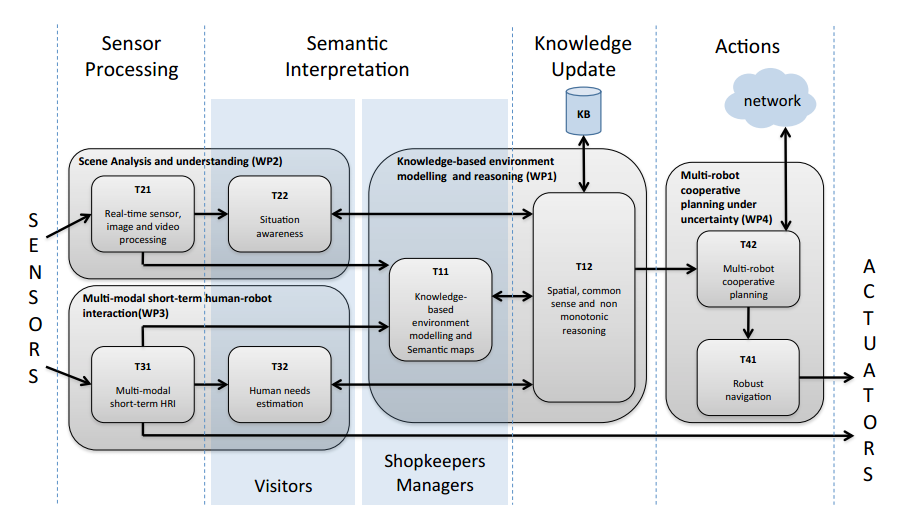
\includegraphics[width=0.9\textwidth]{fig/COACHES_swarch.png}
\caption{\coaches software architecture}
\label{fig:swarch}
\end{figure}

The software architecture of the \coaches robots is shown in Figure \ref{fig:swarch}).
An open architecture (hard/soft) and standard technologies available will be used, 
so that it will be easy to extend and/or adapt the capabilities of the system during the whole length of  the  project  (especially  to  integrate  and  test  various  algorithms  and/or  sensors).  
Such an open architecture will also simplify and optimize integration efficiency as well as re-use of assets in other projects or products. 


%For the development of the software robotics components, the Robot Operating System (ROS)\footnote{www.ros.org}, which is the standard middleware for robotics applications, has been selected.
%ROS provides the middleware infrastructure to effectively share information among the many modules implementing various functionalities on each robot. 
%Moreover, an interface (ROS-through-TCP) will be realized in order to share information among the robots and between ROS and non-ROS components of the system.

The main software components that will be developed for control, reasoning and interaction functionalities of the system are listed below.

\begin{itemize}
\item \emph{Scene analysis}, including sensor processing procedures for both on-board robot devices and static sensors in order to determine the current situation and understand events that are of interest for the system.

\item \emph{Multi-modal HRI}, defining a set of modalities for human-robot interaction, including speech recognition and synthesis, touch interaction, graphical interface on a screen mounted on the robot and Web interfaces.

\item \emph{Knowledge-based representation and reasoning}, defining the formalism and the procedure to represent and reason about the environment and the task of the robots.

\item \emph{Planning and execution monitoring}, for generating the plans to achieve the desired goals and monitor their execution for robust behaviors.

\item \emph{Safe navigation}, for guaranteeing safety operations of the robot in a populated environment.

\end{itemize}

%In the next section we will detail the components 
%\emph{Knowledge-based representation and reasoning} and
%\emph{Planning and execution monitoring},
%where Artificial Intelligence techniques have a fundamental role.



